% Figure 5: HybridDAT Retrieval Flow
% TODO: Replace with actual TikZ diagram showing 3-channel retrieval + dynamic alpha tuning

\begin{figure}[htbp]
\centering
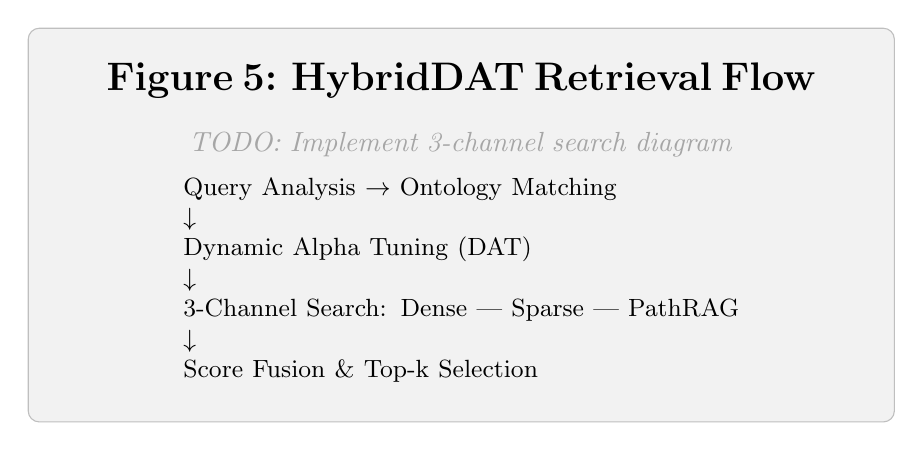
\begin{tikzpicture}
  \node[rectangle, draw=gray!50, fill=gray!10, minimum width=11cm, minimum height=5cm, rounded corners] (placeholder) {};
  \node[text width=10cm, align=center] at (placeholder.center) {
    \textbf{\Large Figure 5: HybridDAT Retrieval Flow}\\[1em]
    \textcolor{gray!70}{\textit{TODO: Implement 3-channel search diagram}}\\[0.5em]
    \small
    \begin{tabular}{l}
    Query Analysis $\rightarrow$ Ontology Matching \\
    $\downarrow$ \\
    Dynamic Alpha Tuning (DAT) \\
    $\downarrow$ \\
    3-Channel Search: Dense | Sparse | PathRAG \\
    $\downarrow$ \\
    Score Fusion \& Top-k Selection \\
    \end{tabular}
  };
\end{tikzpicture}
\caption{HybridDAT retrieval pipeline with dynamic alpha tuning based on query characteristics. The system adjusts weights between dense (FAISS), sparse (TF-IDF), and PathRAG channels according to query type (numeric/disease/practice).}
\label{fig:hybriddat}
\end{figure}
